\section{Fault Interface Conditions}
\label{sec:fault}

Fault interfaces are used to create dislocations (jumps in the
displacement field) in the model. The dislocations arise from slip
across a fault surface. Both shear and tensile dislocations are
supported. For fault interfaces, dislocations in 2D left-lateral-slip and
fault opening, and in 3D left-lateral-slip, reverse-slip, and fault
opening. PyLith supports kinematic (prescribed) slip and dynamic
(spontaneous) rupture simulations.

\userwarning{Spontaneous rupture is not available in PyLith v3.0; we plan
  to have it reimplemented in v3.1.}

\subsection{Conventions}

Slip corresponds to relative motion across a fault surface. Figure
\vref{fig:fault:orientation} shows the orientation of the slip vector
in 3D with respect to the fault surface and coordinate axes. PyLith
automatically determines the orientation of the fault surface. This
alleviates the user from having to compute the strike, dip, and rake
angles over potentially complex, nonplanar fault surfaces. Instead,
the user specifies fault parameters in terms of lateral motion, reverse
motion, and fault opening as shown in Figure \vref{fig:fault:slip:motions}.

\begin{figure}[htbp]
  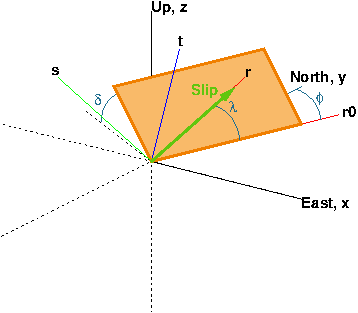
\includegraphics{physics/figs/faultOrientation}
  \caption{Orientation of a fault surface in 3D, where $\phi$ denotes the angle
    of the fault strike, $\delta$ denotes the angle of the fault dip,
    and $\lambda$ the rake angle.}
  \label{fig:fault:orientation} 
\end{figure}

\begin{figure}[htbp]
  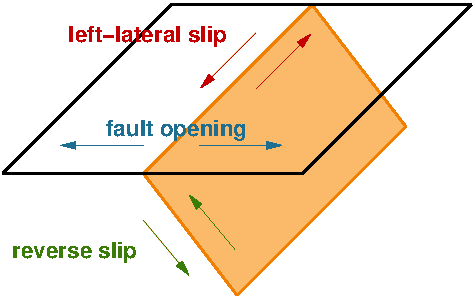
\includegraphics{physics/figs/slipmotions}
  \caption{Sign conventions associated with fault slip. Positive values are associated
    with left-lateral, reverse, and fault opening motions.}
  \label{fig:fault:slip:motions} 
\end{figure}

\subsection{Fault Implementation}

In order to create relative motion across the fault surface in the
finite-element mesh, additional degrees of freedom are added along
with adjustment of the topology of the mesh. These additional degrees
of freedom are associated with cohesive cells. These zero-volume cells
allow control of the relative motion between vertices on the two sides
of the fault. PyLith automatically adds cohesive cells for each fault
surface. Figure \vref{fig:fault:cohesive:cells} illustrates the results
of inserting cohesive cells in a mesh consisting of triangular cells.
This example also shows the distinction between how buried fault edges
are handled differently than fault edges that reach the edge of the
domain, such as the ground surface.

\begin{figure}[htbp]
  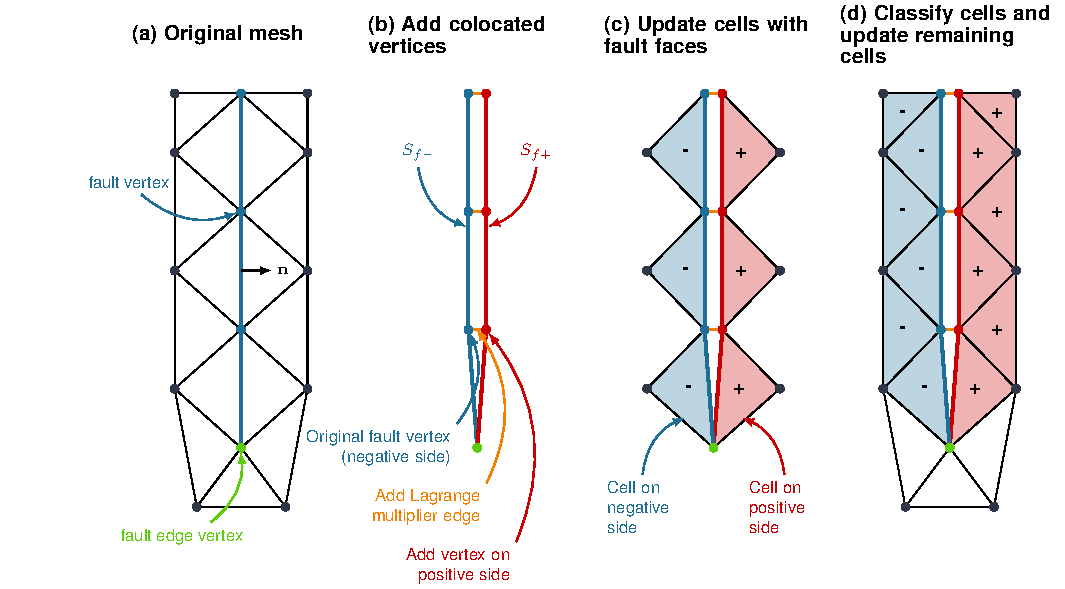
\includegraphics[width=6.25in]{physics/figs/cohesivecell}
  \caption{Example of cohesive cells inserted into a mesh of
    triangular cells.  The zero thickness cohesive cells control slip
    on the fault via the relative motion between the vertices on the
    positive and negative sides of the fault.}
  \label{fig:fault:cohesive:cells} 
\end{figure}

\begin{figure}[htbp]
  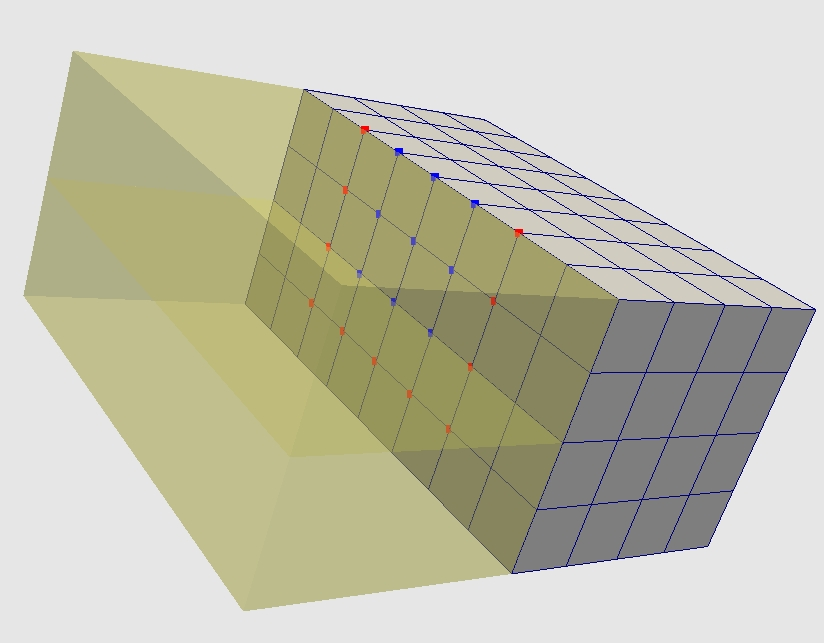
\includegraphics[width=4in]{physics/figs/faultEdge}
  \caption{Example of how faults with buried edges must be described
    with two sets of vertices. All of the vertices on the fault are
    included in the \texttt{fault} group; the subset of vertices along
    the buried edges are included in the \texttt{fault\_edge}
    group. In 2-D the fault edges are just a single vertex as shown in
    Figure
    \vref{fig:fault:cohesive:cells}(a).}
  \label{fig:fault:fault_edge}
\end{figure}
For faults that have buried edges, splitting the mesh apart and inserting
the cohesive cells becomes complex at the buried edges due to the
ambiguity of defining where the fault ends and how to insert the cohesive
cell. In PyLith v2.0.0 we have changed how the buried edges of the
fault are managed. An additional group of fault nodes is specified
(e.g., via a nodeset from CUBIT) that marks the buried edges of the
fault (see Figure \vref{fig:fault:fault_edge}). This allows the cohesive
cell insertion algorithm to adjust the topology so that cohseive cells
are inserted up to the buried edge of the fault but no additional
degrees of freedom are added on the fault edge. This naturally forces
slip to zero along the buried edges.

\subsection{Fault Parameters}

The principal parameters for fault interface conditions are:
\begin{inventory}
\propertyitem{id}{This is an integer identifier for the fault surface. It is
used to specify the \property{material-id} of the cohesive cells in
the mesh. Material identifiers must be unique across all materials and
fault interfaces. Because PyLith creates the cohesive
cells at runtime, there is no correspondence between the \property{id}
property and information in the input mesh like there
is for materials.}
\propertyitem{label}{Name of group of vertices associated with the fault surface.
This label is also used in error and diagnostic reports (default="").}
\propertyitem{edge}{Name of group of vertices marking the buried edges of the
fault (default="").}
\propertyitem{ref\_dir\_1}{First choice for reference direction to discriminate among tangential directions in 3-D (default=[0,0,1]);}
\propertyitem{ref\_dir\_2}{Second choice for reference direction to discriminate among tangential directions in 3-D (default=[0,1,0]);}
\facilityitem{observers}{Observers of boundary condition, e.g., output
  (default=[\object{PhysicsObserver}]):}
\end{inventory}

In 2D the default in-plane slip is left-lateral, so we use the
reference directions to resolve the ambiguity in specifying reverse
slip. In 3D the reference directions are used to resolve the ambiguity
in the along-strike and dip-dir directions.  If the fault plane is
horizontal, then the up-dir corresponds to the reverse-motion on the
+z side of the fault. The only requirement for this direction is that
it not be collinear with the fault normal direction.  The default
value of [0, 0, 1] is appropriate for most 3D problems.


By default the output observers write both diagnostic information
(e.g., fault orientation directions) and the slip at each time step.
The fault coordinate system is shown in Figure
\vref{fig:fault:slip:motions}.  The vectors in the fault coordinate
system can be transformed to the global coordinate system using the
direction vectors in the diagnostic output.

\userwarning{Output of fault orientation information is not yet available
  in this beta release.}
\todo{brad}{Implement output of fault orientation information.}

\subsection{Kinematic Earthquake Rupture (\protect\object{FaultCohesiveKin})}

Kinematic earthquake ruptures use the \object{FaultCohesiveKin} object
to prescribe the slip as a function of time on the fault surface. Slip
may evolve simultaneously over the fault surface instantaneously in a
single time step (as is usually done in quasistatic simulations) or
propagate over the fault surface over hundreds and up to thousands of
time steps (as is usually done in a dynamic simulation).

Multiple earthquake ruptures can be specified on a single fault surface.
This permits repeatedly rupturing the same portion of a fault or combining
earthquake rupture on one subset of the fault surface with steady
aseismic slip on another subset (the two subsets may overlap in both
time and space). A dynamic array of kinematic earthquake rupture components
associates a name (string) with each kinematic rupture. The default
dynamic array contains a single earthquake rupture, ``rupture''. 

\todo{brad}{Add note about discretization of "slip" auxiliary
  subfield.}

\subsubsection{Kinematic Rupture Parameters (\protect\object{KinSrc})}

The kinematic rupture parameters include the origin time and slip
time function. The slip initiation time in the slip time function
is relative to the origin time (default is 0). This means that slip
initiates at a point at a time corresponding to the sum of the kinematic
rupture's origin time and the slip initiation time for that point.

\begin{cfg}[\object{FaultCohesiveKin} parameters in a \filename{cfg} file]
<h>[pylithapp.problem]</h>
<f>interfaces</f> = [fault]
# FaultCohesiveKin is the default for a fault.

<h>[pylithapp.problem.interfaces.fault]</h>
<p>id</p> = 10
<p>label</p> = fault_x
<p>edge</p> = fault_x_buried_edge

# KinSrcStep is the default slip-time function.

<h>[pylithapp.problem.interfaces.fault.eq_ruptures.rupture]</h>
<f>db_auxiliary_field</f> = spatialdata.spatialdb.UniformDB
<p>db_auxiliary_field.label</p> = Fault rupture auxiliary field spatial database
<p>db_auxiliary_field.values</p> = [initiation_time, final_slip_left_lateral, final_slip_opening]
<p>db_auxiliary_field.data</p> = [0.0*s, -2.0*m, 0.0*m]
\end{cfg}

\subsubsection{Slip Time Function}

The current release of PyLith supports specification of the evolution
of fault slip using analytical expressions for the slip time history
at each point, where the parameters for the slip time function may
vary over the fault surface. Currently, two slip time functions are
available: (1) a step-function for quasistatic modeling of earthquake
rupture and (2) a constant slip rate time function for modeling steady
aseismic slip.  Additional slip time functions will likely be
available in future releases. The default slip time function is the
step-function slip function.


\paragraph{Step-Function Slip Time Function (\protect\object{KinSrcStep})}

This slip function prescribes a step in slip at a given time at a
point: 
\begin{gather}
D(t)=\left\{ \begin{array}{cc}
0 & 0\leq t<t_{r}\\
D_{final} & t\ge t_{r}
\end{array}\right.\,,
\end{gather}
where $D(t)$ is slip at time $t$, $D_{final}$ is the final slip,
and $t_{r}$ is the slip initiation time (time when rupture reaches
the location). The slip is specified independently for each of the
components of slip, and the slip and slip starting time may vary over
the fault surface.


\begin{table}[htbp]
  \caption{Values in the auxiliary field spatial database for \object{KinSrcStep}.}
  \label{tab:slip:function:step}
  \begin{tabular}{lp{4.0in}}
    \toprule
    \thead{Subfield} & \thead{Components} \\
    \midrule
    initiation\_time & \textemdash \\
    final\_slip & opening, left\_lateral, reverse \\
    \bottomrule
  \end{tabular}
\end{table}


\paragraph{Constant Slip Rate Slip Time Function (\protect\object{KinSrcConstRate})}

This slip function prescribes a constant slip rate for the evolution
of slip at a point: 
\begin{gather}
  D(t)=\left\{ \begin{array}{cc}
0 & 0\leq t<t_{r}\\
V(t-t_{r}) & t\ge t_{r}
\end{array}\right.\,,
\end{gather}
where $D(t)$ is slip at time $t$, $V$ is the slip rate, and $t_{r}$
is the slip initiation time (time when rupture reaches the location).
The slip rate is specified independently for each of the components
of slip, and the slip rate and slip starting time may vary over the
fault surface.

\begin{table}[htbp]
  \caption{Values in the auxiliary field spatial database for \object{KinSrcConstRate}.}
  \label{tab:slip:function:step}
  \begin{tabular}{lp{4.0in}}
    \toprule
    \thead{Subfield} & \thead{Components} \\
    \midrule
    initiation\_time & \textemdash \\
    slip\_rate & opening, left\_lateral, reverse \\
    \bottomrule
  \end{tabular}
\end{table}


% \paragraph{Liu-Cosine Slip Time Function}

% This slip time function, proposed by Liu, Archuleta, and Hartzell
% for use in ground-motion modeling\cite{Liu:etal:2006}, combines several
% cosine and sine functions together to create a slip time history with
% a sharp rise and gradual termination with a finite duration of slip.
% The evolution of slip at a point follows: 
% \begin{gather}
% D(t)=\left\{ \begin{array}{cc}
% D_{\mathit{final}}C_{n}\left(0.7t-0.7\frac{t_{1}}{\pi}\sin\frac{\pi t}{t_{1}}-1.2\frac{t_{1}}{\pi}\left(\cos\frac{\pi t}{2t_{1}}-1\right)\right) & 0\leq t<t_{1}\\
% D_{\mathit{final}}C_{n}\left(1.0t-0.7\frac{t1}{\pi}\sin\frac{\pi t}{t_{1}}+0.3\frac{t2}{\pi}\sin\frac{\pi(t-t1)}{t_{2}}+\frac{1.2}{\pi}t_{1}-0.3t_{1}\right) & t_{1}\leq t<2t_{1}\\
% D_{\mathit{final}}C_{n}\left(0.7-0.7\cos\frac{\pi t}{t_{1}}+0.6\sin\frac{\pi t}{2t_{1}}\right) & 2t_{1}\leq t\leq t_{0}
% \end{array}\right.\,,\\
% C_{n}=\frac{\pi}{1.4\pi t_{1}+1.2t_{1}+0.3\pi t_{2}},\\
% t_{0}=1.525t_{\mathit{rise}},\\
% t_{1}=0.13t_{0},\\
% t_{2}=t_{0}-t_{1},
% \end{gather}
% where $D(t)$ is slip at time $t$, $D_{final}$ is the final slip
% at the location, $t_{r}$ is the slip initiation time (time when rupture
% reaches the location), and $t_{\mathit{rise}}$ is the rise time.
% \begin{inventory}
% \facilityitem{slip}{Spatial database of final slip distribution ($D_{final})$.}
% \facilityitem{slip\_time}{Spatial database of slip initiation times ($t_{r}$).}
% \facilityitem{rise\_time}{Spatial database for rise time ($t_{\mathit{rise}}$).}
% \end{inventory}
% The spatial database files for the slip time function use the same
% parameters for the slip time function as the Brune slip time function
% shown in Table \vref{tab:slip:function:Brune}.


% \paragraph{Time-History Slip Time Function}

% This slip time function reads the slip time function from a data file,
% so it can have an arbitrary shape. The slip and slip initiation times
% are specified using spatial databases, so the slip time function,
% in general, will use a normalized amplitude.
% \begin{inventory}
% \facilityitem{slip}{Spatial database of final slip distribution ($D_{final})$.}
% \facilityitem{slip\_time}{Spatial database of slip initiation times ($t_{r}$).}
% \facilityitem{time\_history}{Temporal database for slip evolution.}
% \end{inventory}

% \begin{cfg}[\object{TimeHistorySlipFn} parameters in a \filename{cfg} file]
% <h>[pylithapp.problem.interfaces.fault.eq_ruptures.ruptures]</h>
% <f>slip_function</f> = pylith.faults.TimeHistorySlipFn 

% <h>[pylithapp.problem.interfaces.fault.eq_ruptures.rupture.slip_function]</h>
% <p>slip.iohandler.filename</p> = finalslip.spatialdb
% <p>slip_time.iohandler.filename</p> = sliptime.spatialdb
% <p>time_history.iohandler.filename</p> = myfunction.timedb
% \end{cfg}
% The spatial database files for the slip time function specify the
% spatial variation in the parameters for the slip time function, as
% shown in Table \vref{tab:slip:function:Brune-2}.

% \begin{table}[htbp]
% \caption{Values in spatial database used
% as parameters in the time history slip time function.}
% \label{tab:slip:function:Brune-2}
% \begin{tabular}{llp{2.5in}}
% \textbf{Spatial database} & \textbf{Value} & \textbf{Description}\\
% \hline 
% \facility{slip} & \texttt{left-lateral-slip} & Amount of left-lateral final slip in meters. Use negative values for
% right-lateral slip. \\
%  & \texttt{reverse-slip} & Amount of reverse slip in meters. Use negative values for normal slip.
% \\
%  & \texttt{fault-opening} & Amount of fault opening in meters. Negative values imply penetration.\\
% \facility{rise\_time} & \texttt{rise-time} & Rise time ($t_{r})$ in seconds.\\
% \facility{slip\_time} & \texttt{slip-time} & Slip initiation time ($t_{t})$ in meters.\\
% \hline 
% \end{tabular}
% \end{table}


% \subsection{Dynamic Earthquake Rupture}

% Dynamic fault interfaces use the FaultCohesiveDyn object to specify
% a fault constitutive model to govern the fault tractions (friction)
% and the resulting slip. When friction is large enough such that there
% is no sliding on the fault, the fault is locked (slip is zero) and
% the Lagrange multipliers assume their values just as they do in kinematic
% ruptures. In this case, the Lagrange multipliers correspond to the
% forces necessary to keep the slip zero. When the driving forces exceed
% those allowed by friction, we reduce the values of the Lagrange multipliers
% to those consistent with friction from the fault constitutive model.
% When we reduce the Lagrange multipliers, we must increment the slip
% accordingly to maintain consistency in the algebraic system of equations.


% \subsubsection{Fault Constitutive Models}
% \label{sec:fault:constitutive:models}

% PyLith provides four fault constitutive models. Future releases may
% contain additional models, and a template is provided for you to construct
% your own (see Section \vref{sec:extending:fault}).
% The fault constitutive model implementations are independent of dimension
% and work in both 2D and 3D. In solving the governing equations, PyLith
% will use a scalar representation of the shear traction in 2D and a
% vector representation of the shear traction in 3D, with the shear
% traction resolved in the direction of current slip. The fault constitutive
% models contain a common set of properties and components:
% \begin{inventory}
% \propertyitem{label}{Name of the friction model.}
% \facilityitem{db\_properties}{Spatial database of the friction model parameters (default is \object{SimpleDB}).}
% \facilityitem{db\_initial\_state}{Spatial database for initial state variables.
% A warning will be given when a spatial database for the initial state
% is not specified. The default is none which results in initial state
% values of 0.0. For some friction models, we provide more meaningful
% values for default values.}
% \end{inventory}

% \paragraph{Static Friction}

% The static friction model produces shear tractions proportional to
% the fault normal traction plus a cohesive stress,
% \begin{equation}
% T_{f}=\begin{cases}
% T_{c}-\mu_{f}T_{n} & T_{n}\leq0\\
% 0 & T_{n}>0
% \end{cases}.
% \end{equation}
% The spatial database file for the static friction model properties
% specifies the spatial variation of the parameters given in Table \vref{tab:static:friction:properties}.

% \begin{table}[htbp]
% \caption{Values in the spatial database for constant friction parameters.}
% \label{tab:static:friction:properties}
% \begin{tabular}{lp{2.5in}}
% \textbf{Value} & \textbf{Description}\\
% \hline 
% \texttt{friction-coefficient} & Coefficient of friction, $\mu_{f}$\\
% \texttt{cohesion} & Cohesive stress, $T_{c}$\\
% \hline 
% \end{tabular}
% \end{table}


% \paragraph{Slip-Weakening Friction}
% \label{sec:friction:slip:weakening}

% The linear slip-weakening friction model produces shear tractions
% equal to the cohesive stress plus a contribution proportional to the
% fault normal traction that decreases from a static value to a dynamic
% value as slip progresses,
% \begin{equation}
% T_{f}=\begin{cases}
% T_{c}-(\mu_{s}-(\mu_{s}-\mu_{d})\frac{d}{d_{0}})T_{n} & d\leq d_{0}\text{ and }T_{n}\leq0\\
% T_{c}-\mu_{d}T_{n} & d>d_{0}\text{ and }T_{n}\leq0\\
% 0 & T_{n}>0
% \end{cases}
% \end{equation}
% The spatial database files for the slip-weakening friction model properties
% and state variables specify the spatial variation of the fault constitutive
% model parameters given in Table \vref{tab:slip:weakening:properties:statevars}.
% As long as the fault is locked, the initial state variables are zero,
% so specifying the initial state variables for slip-weakening friction
% is rare. The slip-weakening friction also includes a parameter, \property{force\_healing},
% to control healing. In quasistatic simulations, one usually wants
% slip confined to a single time step (\property{force\_healing} = True),
% whereas in a dynamic simulation slip occurs over many time steps (\property{force\_healing}
% = False; default behavior) and fault healing is often neglected. The
% properties include:
% \begin{inventory}
% \propertyitem{force\_healing}{Flag indicating whether healing (cumalative slip
% state variable reset to zero) is forced after every time step.}
% \end{inventory}

% \begin{cfg}[\object{SlipWeakening} parameters in a \filename{cfg} file]
% <h>[pylithapp.problem.interfaces.fault]</h>
% <f>friction</f> = pylith.friction.SlipWeakening ; Change from the default

% <p>friction.force_healing</p> = False ; default value
% \end{cfg}

% \begin{table}[htbp]
% \caption{Values in spatial databases for slip-weakening friction.}
% \label{tab:slip:weakening:properties:statevars}
% \begin{tabular}{llp{2.5in}|}
% \textbf{Spatial database} & \textbf{Value} & \textbf{Description}\\
% \hline 
% \facility{db\_properties} & \texttt{static-coefficient} & Static coefficient of friction, $\mu_{s}$\\
%  & \texttt{dynamic-coefficient} & Dynamic coefficient of friction, $\mu_{d}$\\
%  & \texttt{slip-weakening-parameter} & Slip-weakening parameter, $d_{0}$\\
%  & \texttt{cohesion} & Cohesive stress, $T_{c}$\\
% \facility{db\_initial\_state} & \texttt{cumulative-slip} & Cumulative slip, $d$\\
%  & \texttt{previous-slip} & Slip at previous time step, $d(t-\Delta t)$\\
% \hline 
% \end{tabular}
% \end{table}


% \paragraph{Time-Weakening Friction}

% The linear time-weakening friction model is analogous to the linear
% slip-weakening friction model with time replacing slip. It produces
% shear tractions equal to the cohesive stress plus a contribution proportional
% to the fault normal traction that decreases from a static value to
% a dynamic value as time progresses,
% \begin{equation}
% T_{f}=\begin{cases}
% T_{c}-(\mu_{s}-(\mu_{s}-\mu_{d})\frac{t}{t_{0}})T_{n} & t\leq t_{0}\text{ and }T_{n}\leq0\\
% T_{c}-\mu_{d}T_{n} & t>t_{0}\text{ and }T_{n}\leq0\\
% 0 & T_{n}>0
% \end{cases}
% \end{equation}
% The spatial database files for the time-weakening friction model properties
% and state variables specify the spatial variation of the fault constitutive
% model parameters given in Table \vref{tab:time:weakening:properties:statevars}.
% As long as the fault is locked, the initial state variable is zero,
% so specifying the initial state variable for time-weakening friction
% is rare.

% \begin{table}[htbp]
% \caption{Values in spatial databases for time-weakening friction.}
% \label{tab:time:weakening:properties:statevars}
% \begin{tabular}{llp{2.5in}}
% \textbf{Database} & \textbf{Value} & \textbf{Description}\\
% \hline 
% \facility{db\_properties} & \texttt{static-coefficient} & Static coefficient of friction, $\mu_{s}$\\
%  & \texttt{dynamic-coefficient} & Dynamic coefficient of friction, $\mu_{d}$\\
%  & \texttt{time-weakening-parameter} & Time-weakening parameter, $t_{0}$\\
%  & \texttt{cohesion} & Cohesive stress, $T_{c}$\\
% \facility{db\_initial\_state} & \texttt{elapsed-time} & Elasped time of slip, $t$\\
% \hline 
% \end{tabular}
% \end{table}


% \paragraph{Slip- and Time-Weakening Friction I}
% \label{sec:friction:slip:time:weakening}

% This friction model, used in a few SCEC Spontaneous Rupture benchmarks,
% combines characteristics of slip-weakening and time-weakening friction.
% The time-weakening portion is generally used to force nucleation of
% the rupture. The model produces shear tractions equal to the cohesive
% stress plus a contribution proportional to the fault normal traction
% that decreases from a static value to a dynamic value as slip progresses
% or when a weakening time is reached,
% \begin{equation}
% T_{f}=\begin{cases}
% T_{c}-(\mu_{s}-(\mu_{s}-\mu_{d})\frac{d}{d_{0}})T_{n} & d\leq d_{0}\text{ and }t<t_{w}\text{ and }T_{n}\leq0\\
% T_{c}-\mu_{d}T_{n} & (d>d_{0}\text{ or }t\ge t_{w})\text{ and }T_{n}\leq0\\
% 0 & T_{n}>0
% \end{cases}
% \end{equation}
% The spatial database files for the slip- and time-weakening friction
% model properties and state variables specify the spatial variation
% of the fault constitutive model parameters given in Table \vref{tab:slip:time:weakening:properties:statevars}.
% As long as the fault is locked, the initial state variables are zero,
% so specifying the initial state variables for slip-weakening friction
% is rare. This variation of slip-weakening friction does not include
% the \texttt{force\_healing} parameter, because this friction model
% was developed for dynamic simulations.

% \begin{cfg}[\object{SlipWeakeningTime} parameters in a \filename{cfg} file]
% <h>[pylithapp.problem.interfaces.fault]</h>
% <f>friction</f> = pylith.friction.SlipWeakeningTime ; Change from the default
% \end{cfg}

% \begin{table}[htbp]
% \caption{Values in spatial databases for a simple slip- and time-weakening friction model.}
% \label{tab:slip:time:weakening:properties:statevars}
% \begin{tabular}{llp{2.5in}}
% \textbf{Spatial database} & \textbf{Value} & \textbf{Description}\\
% \hline 
% \facility{db\_properties} & \texttt{static-coefficient} & Static coefficient of friction, $\mu_{s}$\\
%  & \texttt{dynamic-coefficient} & Dynamic coefficient of friction, $\mu_{d}$\\
%  & \texttt{slip-weakening-parameter} & Slip-weakening parameter, $d_{0}$\\
%  & \texttt{weakening-time} & Weakening time, $t_{w}$\\
%  & \texttt{cohesion} & Cohesive stress, $T_{c}$\\
% \facility{db\_initial\_state} & \texttt{cumulative-slip} & Cumulative slip, $d$\\
%  & \texttt{previous-slip} & Slip at previous time step, $d(t-\Delta t)$\\
% \hline 
% \end{tabular}
% \end{table}


% \paragraph{Slip- and Time-Weakening Friction II}
% \label{sec:friction:slip:time:stable:weakening}

% This friction model, used in a few SCEC Spontaneous Rupture benchmarks,
% merges features of slip-weakening and time-weakening to provide a
% more numerically stable version of the Slip- and Time-Weakening Friction
% I model. Rather than an instantaneous drop in the coefficient of friction
% from the static value to the dynamic value when the weakening time
% is reached, the weakening progresses linearly with time. As in the
% other slip- and time-weakening friction model, the time-weakening
% portion is generally used to force nucleation of the rupture. The
% model produces shear tractions equal to the cohesive stress plus a
% contribution proportional to the fault normal traction that decreases
% from a static value to a dynamic value as slip and time progress,
% \begin{equation}
% T_{f}=\begin{cases}
% T_{c}-(\mu_{s}-(\mu_{s}-\mu_{d})max(f_{1},f_{2}))T_{n} & T_{n}\leq0\\
% 0 & T_{n}>0
% \end{cases}
% \end{equation}
% \begin{equation}
% f_{1}=\begin{cases}
% d/d_{0} & d\leq d_{0}\\
% 1 & d\ge d_{0}
% \end{cases}
% \end{equation}
% \begin{equation}
% f_{2}=\begin{cases}
% 0 & t\leq t_{w}\\
% (t-t_{w})/t_{0} & t_{w}<t\le t_{w}+t_{0}\\
% 1 & t>t_{w}+t_{0}
% \end{cases}
% \end{equation}
% The spatial database files for the slip- and time-weakening friction
% model properties and state variables specify the spatial variation
% of the fault constitutive model parameters given in Table \vref{tab:slip:time:stable:weakening:properties:statevars}.
% As long as the fault is locked, the initial state variables are zero,
% so specifying the initial state variables for slip-weakening friction
% is rare. This variation of slip-weakening friction does not include
% the \texttt{force\_healing} parameter, because this friction model
% was developed for dynamic simulations.

% \begin{cfg}[\object{SlipWeakeningTimeStable} parameters in a \filename{cfg} file]
% <h>[pylithapp.problem.interfaces.fault]</h>
% <f>friction</f> = pylith.friction.SlipWeakeningTimeStable ; Change from the default
% \end{cfg}

% \begin{table}[htbp]
% \caption{Values
% in spatial databases for a second slip- and time-weakening friction model.}
% \label{tab:slip:time:stable:weakening:properties:statevars}
% \begin{tabular}{llp{2.5in}}
% \textbf{Spatial database} & \textbf{Value} & \textbf{Description}\\
% \hline 
% \facility{db\_properties} & \texttt{static-coefficient} & Static coefficient of friction, $\mu_{s}$\\
%  & \texttt{dynamic-coefficient} & Dynamic coefficient of friction, $\mu_{d}$\\
%  & \texttt{slip-weakening-parameter} & Slip-weakening parameter, $d_{0}$\\
%  & \texttt{time-weakening-time} & Weakening time, $t_{w}$\\
%  & \texttt{time-weakening-parameter} & Time-weakening parameter, $t_{0}$\\
%  & \texttt{cohesion} & Cohesive stress, $T_{c}$\\
% \facility{db\_initial\_state} & \texttt{cumulative-slip} & Cumulative slip, $d$\\
%  & \texttt{previous-slip} & Slip at previous time step, $d(t-\Delta t)$\\
% \hline 
% \end{tabular}
% \end{table}


% \paragraph{Rate- and State-Friction with Ageing Law}
% \label{sec:friction:rate:state:ageing}

% The Dieterich-Ruina rate and state friction model produces shear tractions
% equal to the cohesive stress plus a contribution proportional to the
% fault normal traction that depends on a state variable,
% \begin{gather}
% T_{f}=\begin{cases}
% T_{c}-\mu_{f}T_{n} & T_{n}\leq0\\
% 0 & T_{n}>0
% \end{cases}\\
% \mu_{f}=\begin{cases}
% \mu_{0}+a\ln\left(\frac{V}{V_{0}}\right)+b\ln\left(\frac{V_{0}\theta}{L}\right) & V\ge V_{\mathit{linear}}\\
% \mu_{0}+a\ln\left(\frac{V_{linear}}{V_{0}}\right)+b\ln\left(\frac{V_{0}\theta}{L}\right)-a\left(1-\frac{V}{V_{linear}}\right) & V<V_{linear}
% \end{cases}\\
% \frac{d\theta}{dt}=1-\frac{V\theta}{L}
% \end{gather}
% where $V$ is slip rate, $V_{linear}$ is a cutoff for a linear slip
% rate dependence, $a$ and $b$ are coefficients, $L$ is the characteristic
% slip distance, $\theta$ is a state variable. With an interative solver
% in quasistatic simulations with its small, but nonzero residual tolerance
% we never encounter zero slip rates in quasistatic simulations. Instead
% we want to avoid significant variations in the coefficient of friction
% for slip rates on the same order as our residual tolerance. We regularize
% the rate and state friction model by imposing a linearization of the
% variation of the coefficient of friction with slip rate when the slip
% rate drops below a cutoff slip rate, $V_{linear}$ (\property{linear\_slip\_rate}
% property with a default value of 1.0e-12). Note that this is different
% than the popular inverse hyperbolic sine regularization proposed by
% Ben-Zion and Rice \cite{BenZion:Rice:1997} to permit zero slip rates.
% Following Kaneko \textit{et al.} \cite{Kaneko:etal:2008}, we integrate
% the evolution equation for the state variable, keeping slip rate constant,
% to get
% \begin{equation}
% \theta(t+\Delta t)=\theta(t)\exp\left(\frac{-V(t)\Delta t}{L}\right)+\frac{L}{V(t)}\left(1-\exp\left(-\frac{V(t)\Delta t}{L}\right)\right).
% \end{equation}
% As the slip rate approaches zero, the first exponential term approaches
% 1. Using the first three terms of the Taylor series expansion of the
% second exponential yields
% \begin{equation}
% \theta(t+\Delta t)=\begin{cases}
% \theta(t)\exp\left(-\frac{V(t)\Delta t}{L}\right)+\Delta t-\frac{1}{2}\frac{V(t)\Delta t^{2}}{L} & \frac{V(t)\Delta t}{L}<0.00001\\
% \theta(t)\exp\left(-\frac{V(t)\Delta t}{L}\right)+\frac{L}{V(t)}\left(1-\exp\left(-\frac{V(t)\Delta t}{L}\right)\right) & \frac{V(t)\Delta t}{L}\ge0.00001
% \end{cases}
% \end{equation}

% A zero value for the initial state results in infinite values for
% the coefficient of friction. To avoid such behavior when the user
% fails to provide nonzero values for the initial state, we set the
% state variable to $L/V_{0}$.

% The properties include:
% \begin{inventory}
% \propertyitem{linear\_slip\_rate}{Nondimensional slip rate at which linearization
% occurs, $V_{linear}$. In quasistatic simulations it should be about
% one order of magnitude larger than absolute tolerance in solve.}
% \end{inventory}

% \begin{cfg}[\object{RateStateAgeing} parameters in a \filename{cfg} file]
% <h>[pylithapp.problem.interfaces.fault]</h>
% <f>friction</f> = pylith.friction.RateStateAgeing ; Change from the default
% <p>friction.linear_slip_rate</p> = 1.0e-12 ; default value
% \end{cfg}
% The spatial database files for the rate- and state-friction model
% properties and state variables specify the spatial variation of the
% fault constitutive model parameters given in Table \vref{tab:rate:state:ageing:properties:statevars}.

% \begin{table}[htbp]
% \caption{Values in spatial databases for Dieterich-Ruina rate-state friction.}
% \label{tab:rate:state:ageing:properties:statevars}
% \begin{tabular}{llp{2.5in}}
% \textbf{Database} & \textbf{Value} & \textbf{Description}\\
% \hline 
% \facility{db\_properties} & \texttt{reference-friction-coefficient} & Steady-state coefficient of friction at slip rate $V_{0}$, $\mu_{s}$\\
%  & \texttt{reference-slip-rate} & Reference slip rate, $V_{0}$\\
%  & \texttt{characteristic-slip-distance} & Slip-weakening parameter, $L$\\
%  & \texttt{constitutive-parameter-a} & Coefficient for the $\ln$ slip rate term, $a$\\
%  & \texttt{constitutive-parameter-b} & Coefficient for the $\ln$ state variable term, $b$\\
%  & \texttt{cohesion} & Cohesive stress, $T_{c}$\\
% \facility{db\_initial\_state} & \texttt{state-variable} & State variable, $\theta$\\
% \hline 
% \end{tabular}
% \end{table}


% \subsection{Slip Impulses for Green's Functions}
% \label{sec:fault:cohesive:impulses}

% Computing static Green's functions using the \object{GreensFns} problem requires
% a specialized fault implementation, \object{FaultCohesiveImpulses}, to set
% up the slip impulses. The parameters controlling the slip impulses
% include the components involved (lateral, reverse, and/or fault opening)
% and the amplitude of the pulses (e.g., selecting a subset of a fault
% or including a spatial variation). The \object{FaultCohesiveImpulses} properties and facilities
% include:
% \begin{inventory}
% \propertyitem{threshold}{Threshold for non-zero amplitude; impulses will only
% be generated at locations on the fault where the amplitude exceeds
% this threshold.}
% \propertyitem{impulse\_dof}{Array of components associated with impulses, e.g.,
% [0, 1, 2] for slip involving the left-lateral, reverse, and opening
% components, respectively.}
% \facilityitem{db\_impulse\_amplitude}{Spatial database for amplitude of slip
% impulse (scalar field). Default is \object{SimpleDB}.}
% \end{inventory}

% \begin{cfg}[\object{FaultCohesiveImpulses} parameters in a \filename{cfg} file]
% <h>[pylithapp.problem.interfaces]</h>
% <f>fault</f> = pylith.faults.FaultCohesiveImpulses ; Change from the default 

% <h>[pylithapp.problem.interfaces.fault]</h>
% <p>threshold</p> = 1.0e-6*m ; default
% <p>impulse_dof</p> = [0] ; lateral slip-only
% <p>db_impulse_amplitude.iohandler.filename</p> = myimpulse.spatialdb
% <p>db_impulse_amplitude.label</p> = Impulse amplitude
% \end{cfg}


% End of file
